\input{../mac/head-default.tex}
\input{../mac/maths.tex}

\usepackage{tikz}
\usetikzlibrary{automata,decorations.markings}
\newcommand*{\pt}{5mm}

\Bdc{Notes on the Theory of Computation}

\section{Automata and Formal Languages}

An {\bf alphabet} is a finite set \(\varSigma\), and a {\bf word over the
alphabet \(\varSigma\)} is a finite sequence or {\bf string} of the elements of
\(\varSigma\). If a word \(w\) is the sequence \((w_0, \ldots, w_n)\) for some
\(n \in \setnat\), we may write the word as \(w_0 \cdots w_n\). The empty word
is denoted by \(\varepsilon\). The set of all words over \(\varSigma\) is
\(\varSigma^*\)\footnote{\(^*\) is the unary operator of Kleene star, defined
as \(A^* = \set{a_0 \cdots a_n : n \in \setnat \land \forall \, i \in \Nln[n +
1] \, (a_i \in A)}\).}. A {\bf formal language over the alphabet \(\varSigma\)}
is a subset of \(\varSigma^*\).

An {\bf automaton} is an ordered sequence that {\bf accepts} some words over an
alphabet. The set of words an automaton accepts forms a language, which is
unique, in which case we say the automaton {\bf recognises} the language. Given
an automaton \(M\), we may speak of the unique language recognised by \(M\) as
the {\bf language of the automaton \(M\)} and denote it by \(L(M)\). An
automaton may accept no string, in which case the language thereof is \(\nset\).

\subsection{Finite-State Automata and Regular Languages}

\Bdf
    A {\bf deterministic finite-state automaton} is an ordered quintuple
    \((\varSigma, S, \delta, s_0, F)\) wherein
    \begin{enumerate}
        \item \(\varSigma\) is an alphabet,
        \item \(S\) is a finite set of {\bf states},
        \item \(\map{\delta}{S \times \varSigma}{S}\) is the {\bf transition
        function},
        \item \(s_0 \in S\) is the {\bf initial state}, and
        \item \(F \subseteq S\) is the set of {\bf final states} or {\bf
        accepting states}.
    \end{enumerate}
\Edf

Let \(M = (\varSigma, S, \delta, s_0, F)\) be a deterministic finite-state
automaton and let \(w = w_0 \cdots w_n\) wherein \(n \in \setnat\) be a word
over \(\varSigma\).  Then \(M\) accepts \(w\) if there exists a finite sequence
of states \((r_0, \ldots, r_{n + 1})\) in \(S\) such that
\begin{enumerate}
    \item \(r_0 = s_0\),
    \item \(\delta(r_i, w_i) = r_{i + 1}\) for \(i = 0, \ldots, n\), and
    \item \(r_{n + 1} \in F\).
\end{enumerate}

\Bdf
    A {\bf nondeterministic finite-state automaton} is an ordered quintuple
    \((\varSigma, S, \delta, s_0, F)\) wherein
    \begin{enumerate}
        \item \(\varSigma\) is an alphabet,
        \item \(S\) is a finite set of states,
        \item \(\map{\delta}{S \times
        \varSigma_\varepsilon}{\pow(S)}\)\footnote{\(\varSigma_\varepsilon\)
        denotes the union of \(\varSigma\) and \(\set{\varepsilon}\).} is the
        transition function,
        \item \(s_0 \in S\) is the initial state, and
        \item \(F \subseteq S\) is the set of final or accepting states.
    \end{enumerate}
\Edf

Let \(M = (\varSigma, S, \delta, s_0, F)\) be a nondeterministic finite-state
automaton and let \(w\) be a word over \(\varSigma\). Then \(M\) accepts \(w\)
if \(w = w_0 \cdots w_n\) wherein \(n \in \setnat\) such that each \(w_i \in
\varSigma_\varepsilon\), \(i \in \Nln[n + 1]\), and that there exists a finite
sequence of states \((r_0, \ldots, r_{n + 1})\) in \(S\) such that
\begin{enumerate}
    \item \(r_0 = s_0\),
    \item \(r_{i + 1} \in \delta(r_i, w_i)\) for \(i = 0, \ldots, n\), and
    \item \(r_{n + 1} \in F\)
\end{enumerate}

We say that two automata are equivalent if they recognise the same language.

\Bth
    Every nondeterministic finite-state automaton has an equivalent
    deterministic finite-state automaton.
\Eth
\Bpr
    Let \(N = (\varSigma, S, \delta, s_0, F)\) be the nondeterministic
    finite-state automaton recognising some language \(A\). We construct a
    deterministic finite-state automaton \(M = (\varSigma, S', \delta', s_0',
    F)\) recognising \(A\).

    We first see that \(S' = \pow(S)\) and that \(F' = \set{R \in S' : R \cap F
    \neq \nset}\).

    Let \(\map{\delta_0}{S \times \set{\varepsilon}}{\pow(S)}\) be defined as
    \(\delta_0(s, \varepsilon) = \delta(s, \varepsilon)\) for each \(s \in S\).
    Assume first that, thus induced, \(\delta_0 = \nset\) for \(N\). For each
    \(R \in S'\) and for each \(a \in \varSigma\), let \(\delta'(R, a) = \set{s
    \in S : \exists \, r \in R \, (s \in \delta(r, a))}\). Equivalently,
    \[
        \delta'(R, a) = \bigcup_{r \in R} \delta(r, a).
    \]
    Also let \(s_0' = \set{s_0'}\). We then see that \(M = (\varSigma, S',
    \delta', s_0', F')\) recognises \(A\).

    Assume then that \(\delta_0 \neq \nset\) for \(N\). For each \(R \subseteq S
    \), let
    \[
        E(R) = \set*{s \in S : \exists \, n \in \setnat \, \exists \, r \in R \,
        \big(s = \delta^n(r, \varepsilon)\big)}.
    \]
    We then let
    \[
        \delta'(R, a) = \set*{s \in S : \exists \, r \in R \, s \in
        E\big(\delta(r, a)\big)}
    \]
    and let \(s_0' = E(\set{s_0})\). We similarly see that \(M = (\varSigma, S',
    \delta', s_0' F')\) recognises \(A\).

    Therefore, the theorem holds.
\Epr

\Bdf
    Let \(\varSigma\) be an alphabet, and let \(a \in \varSigma\). Then some \(R
    \subseteq \varSigma^*\) is a {\bf regular language} if
    \begin{enumerate}
        \item \(R = \nset\),
        \item \(R = \set{\varepsilon}\),
        \item \(R = \set{a}\),
        \item \(R = R_1 \cup R_2\) wherein \(R_1\) and \(R_2\) are regular
        languages over \(\varSigma\),
        \item \(R = R_1 R_2\)\footnote{\(R_1 R_2\) is the concatenation of
        \(R_1\) and \(R_2\), defined as \(R_1 R_2 = \set{x y : x \in R_1 \land y
        \in R_2}\)} wherein \(R_1\) and \(R_2\) are regular languages over
        \(\varSigma\), or
        \item \(R = R_0^*\) wherein \(R_0\) is a regular language over
        \(\varSigma\).
    \end{enumerate}
\Edf

An expression used to describe a regular language is a {\bf regular expression}.
If \(R\) is a regular expression, we denote the regular language it describes by
\(L(R)\).

\Blm
    \label{lem1}
    If a language is regular, then some nondeterministic finite-state automaton
    recognises it.
\Elm
\Bpr
    Let \(\varSigma\) be an alphabet, and let \(R\) be a regular language over
    \(\varSigma\). If \(R = \nset\), then the nondeterministic finite-state
    automaton characterised by the following diagram recognises it.
    \begin{figure}[!h]
        \centering
        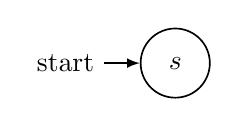
\begin{tikzpicture}[
            ->,>=latex,auto,semithick,
            node distance=2.5cm
        ]
        \node[initial,state] (s) {\(s\)};
        \end{tikzpicture}
    \end{figure}

    \noindent Equivalently, \(N = (\varSigma, \set{s}, \delta, s, \nset)\)
    wherein \(\delta(r, b) = \nset\) for any \(r \in \set{s}\) and for any \(b
    \in \varSigma\) recognises \(R\).

    If \(R = \set{\varepsilon}\), then the nondeterministic finite-state
    automaton characterised by the following diagram recognises it.
    \begin{figure}[!h]
        \centering
        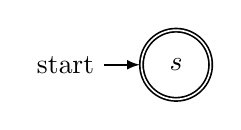
\begin{tikzpicture}[
            ->,>=latex,auto,semithick,
            node distance=2.5cm
        ]
        \node[initial,state,accepting] (s) {\(s\)};
        \end{tikzpicture}
    \end{figure}

    \noindent Equivalently, \(N = (\varSigma, \set{s}, \delta, s, \set{s})\)
    wherein \(\delta(r, b) = \nset\) for any \(r \in \set{s}\) and for any \(b
    \in \varSigma\) recognises \(R\).

    If \(R = \set{a}\) for some \(a \in \varSigma\), then the nondeterministic
    finite-state automaton characterised by the following diagram recognises it.
    \begin{figure}[!h]
        \centering
        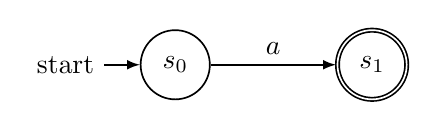
\begin{tikzpicture}[
            ->,>=latex,auto,semithick,
            node distance=2.5cm
        ]
        \node[initial,state] (s0) {\(s_0\)};
        \node[state,accepting] (s1) [right of=s0] {\(s_1\)};
        \path (s0) edge node {\(a\)} (s1);
        \end{tikzpicture}
    \end{figure}

    \noindent Equivalently, \(N = (\varSigma, \set{s_0, s_1}, \delta, s_0,
    \set{s_1})\) wherein \(\delta(s_0, a) = \set{s_1}\) and \(\delta(r, b) =
    \nset\) if \(r \neq s_0\) or \(b \neq a\).

    Assume that \(R_1\) and \(R_2\) are regular languages over \(\varSigma\),
    that \(N_1 = (\varSigma, S_1, \delta_1, s_1, F_1)\) is a nondeterministic
    finite-state automaton recognising \(R_1\), and that \(N_2 = (\varSigma,
    S_2, \delta_2, s_2, F_2)\) is a nondeterministic finite-state automaton
    recognising \(R_2\).

    If \(R = R_1 \cup R_2\), let \(s_0\) be a state not in \(S_1\) or \(S_2\),
    let \(S = \set{s_0} \cup S_1 \cup S_2\), and let \(F = F_1 \cup F_2\).
    Define \(\map{\delta}{S \times \varSigma}{\pow(S)}\) so that for each \(r
    \in S\) and for each \(b \in \varSigma\) we have
    \[
        \delta(r, b) = \begin{cases}
            \delta_1(r, b) & \text{if }\ r \in S_1,\\
            \delta_2(r, b) & \text{if }\ r \in S_2,\\
            \set{s_1, s_2} & \text{if }\ r = s_0 \land b = \varepsilon \text{,
            and}\\
            \nset & \text{otherwise.}
        \end{cases}
    \]
    We see that \(N = (\varSigma, S, \delta, s_0, F)\) is a nondeterministic
    finite-state automaton recognising \(R\).

    If \(R = R_1 R_2\), let \(S = S_1 \cup S_2\). Define \(\map{\delta}{S \times
    \varSigma}{S}\) so that for each \(r \in S\) and for each \(b \in
    \varSigma\) we have
    \[
        \delta(r, b) = \begin{cases}
            \delta_1(r, b) & \text{if }\ (r \in S_1 \land r \not\in F_1) \lor (r
            \in F_1 \land b \neq \varepsilon),\\
            \delta_1(r, b) \cup \set{s_2} & \text{if }\ r \in F_1 \land b =
            \varepsilon \text{, and}\\
            \delta_2(r, b) & \text{otherwise.}
        \end{cases}
    \]
    We see that \(N = (\varSigma, S, \delta, s_1, F_2)\) is a nondeterministic
    finite-state automaton recognising \(R\).

    If \(R = R_1^*\), let \(s_0\) be a state not in \(S_1\), let \(S = \set{s_0}
    cup S_1\), and let \(F = \set{s_0} \cup F_1\). Define \(\map{\delta}{S
    \times \varSigma}{S}\) so that for each \(r \in S\) and for each \(b \in
    \varSigma\) we have
    \[
        \delta(r, b) = \begin{cases}
            \delta_1(r, b) & \text{if }\ (r \in S_1 \land r \not\in F_1) \lor (r
            \in F_1 \land b \neq \varepsilon),\\
            \delta_1(r, b) \cup \set{s_1} & \text{if }\ r \in F_1 \land b =
            \varepsilon,\\
            \set{s_1} & \text{if }\ r = s_0 \land b = \varepsilon \text{, and}\\
            \nset & \text{otherwise.}
        \end{cases}
    \]
    We see that \(N = (\varSigma, S, \delta, s_0, F)\) is a nondeterministic
    finite-state automaton recognising \(R\).

    Therefore, the lemma holds by the principle of induction.
\Epr

\Bdf
    A {\bf generalised nondeterministic finite-state automaton} is an ordered
    quintuple \((\varSigma, S, \delta, s_0, s_1)\) wherein
    \begin{enumerate}
        \item \(\varSigma\) is an alphabet,
        \item \(S\) is a finite set of states,
        \item \(\map{\delta}{(S \setminus \set{s_1}) \times (S \setminus
        \set{s_0})}{\mathcal{R}}\) wherein \(\mathcal{R}\) is the set of all
        regular expressions over \(\varSigma\) is the transition function,
        \item \(s_0 \in S\) is the initial state, and
        \item \(s_1 \in S\) is the final or accepting state.
    \end{enumerate}
\Edf

Let \(M = (\varSigma, S, \delta, s_0, s_1)\) be a generalised nondeterministic
finite-state automaton and let \(w\) be a word over \(\varSigma\). Then \(M\)
accepts \(w\) if \(w = w_0 \cdots w_n\) wherein \(n \in \setnat\) such that each
\(w_i \in \varSigma^*\), \(i \in \Nln[n + 1]\), and that there exists a finite
sequence of states \((r_0, \ldots, r_{n + 1})\) such that
\begin{enumerate}
    \item \(r_0 = s_0\),
    \item \(r_{n + 1} = s_1\), and
    \item for each \(i\) we have \(w_i \in L(R_i)\) wherein \(R_i = \delta(r_i,
    r_{i + 1})\).
\end{enumerate}

\Blm
    \label{lem2}
    If a nondeterministic finite-state automaton recognises a language, then it
    is regular.
\Elm
\Bpr
    Let \(N\) be a nondeterministic finite-state automaton. We prove that
    \(L(N)\) is described by some regular expression \(R\) over \(\varSigma\).

    TODO
\Epr

\Bth
    A language is regular if and only if some nondeterministic finite-state
    automaton recognises it.
\Eth
\Bpr
    The theorem holds by Lemma~\ref{lem1} and Lemma~\ref{lem2}.
\Epr

\Edc